\documentclass[a4paper,oneside]{book}
\usepackage[a4paper]{geometry}
\usepackage[utf8]{inputenc}
\usepackage[T1]{fontenc}
\usepackage{graphicx}
\usepackage{amssymb}
\usepackage{float}
\usepackage{booktabs}
\usepackage{amsmath}
\usepackage{tikz}
\usepackage{subcaption}
\usepackage{bm}
\usetikzlibrary{arrows.meta, positioning}
\newtheorem{definition}{Definition}
\newtheorem{remark}{Remark}
\newtheorem{dimostration}{Dimostration}
\begin{document}

\begin{titlepage}
    \noindent
    \begin{minipage}[c]{0.20\textwidth}
        
\includegraphics[width=\textwidth]{logo_unimib.png}
    \end{minipage}

    \hspace{0.5cm}

    \begin{minipage}[c]{0.75\textwidth}
        {\large\textsc{Università degli Studi di Milano Bicocca}} \\
        {\normalsize Scuola di Scienze} \\
        {\normalsize Dipartimento di Informatica, Sistemistica e Comunicazione} \\

        \textbf{Corso di Laurea in Informatica}
    \end{minipage}

    \vfill

    \begin{center}
        {\LARGE\textbf{Appunti Causal Networks}}
    \end{center}

    \vfill
    \vspace{15mm}

    \vfill

    \begin{center}
        {\large\bfseries Anno Accademico 2026-2027}
    \end{center}

\end{titlepage}
\tableofcontents

\newpage 
\chapter{Introduction to Causal Networks}
With the term Artificial Intelligence (\textbf{AI}) we refer to the intelligence demonstrated by machines that mimic cognitive functions that humans associate with other human minds, such as learning and problem-solving.
Machine learning (\textbf{ML}) is a subset of AI compound by algorithms and statistical models that computer systems use to perform specific tasks without using explicit instructions, relying on patterns and inference instead.
There are 3 types of ML: supervised learning, self-supervised (or unsupervised learning) and reinforcement learning.
Deep Learning (\textbf{DL}) is a subset of ML that uses artificial neural networks to model and understand complex patterns and relationships in data.
Anyway, everything is based on curve fitting, linear or non-linear, and the goal is to minimize the error between the predicted output and the actual output.
For this reason, studying the causation is important to make sense of data, to understand how to have an effect on a system and to guide actions and policies.
In the Figure \ref{fig:ai_set.png} you can see the relationship between AI, ML and DL.

\begin{figure}[ht]
    \centering
    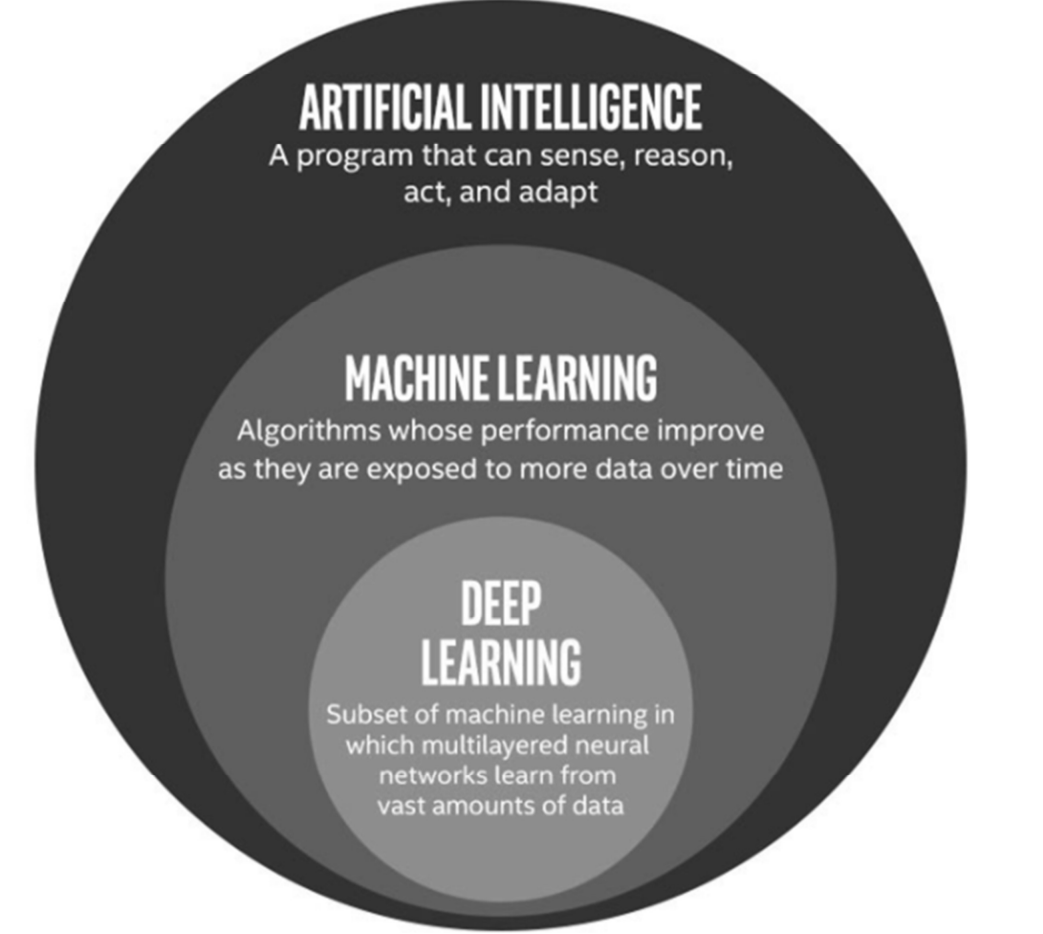
\includegraphics[width=0.6\textwidth]{immagini/ai_set.png}
    \caption{The set of AI, ML and DL.}
    \label{fig:ai_set.png}
\end{figure}

\section{Simpson's Paradox}
\label{simp_para_cap}
Statistical phenomenon in which an observed trend in different groups disappears or reverses when the groups are combined, so this can lead to an evaluation error.
So data alone aren't enough to fully understand a system and  to make decisions (\textbf{correlation is not causation}).
In Fig. \ref{fig:simp_para_exe.png} there is an example, if we consider only the combined data the drug appears to be harmful: only 78\% of the patients recovered 
compared to 83\% of the patients that didn't take the drug, but if we consider the data divided by gender, we can see that the drug is actually beneficial for both men and women.
\begin{figure}[ht]
    \centering
    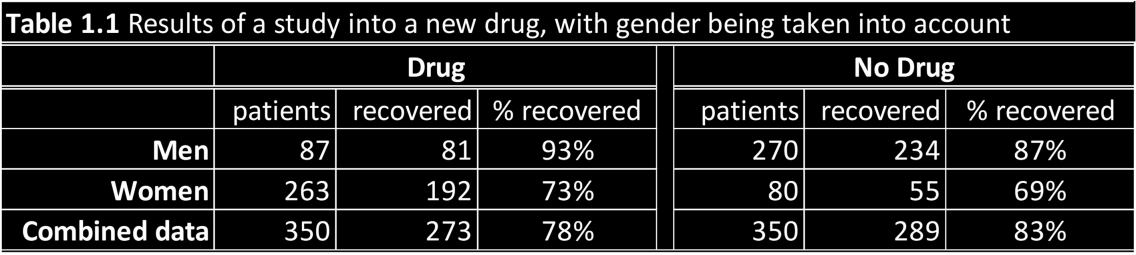
\includegraphics[width=0.6\textwidth]{immagini/simp_para_exe.png}
    \caption{Simpson's Paradox - Example.}
    \label{fig:simp_para_exe.png}
\end{figure}

\subsection{The Pitfall of Blind Data Segregation}

A common mistake is assuming that segregating data by any available variable always yields 
the correct decision. 
\newline
Indeed, as shown in the following example (Fig \ref{fig:simp_para_exe2.png}) is not correct to just segregate the data whenever is possible. 
In this example we were considering the effect of a drug on the recovery of patients with an High BP by lowering the BP, unfortunately the drug has also a toxic effect.
The segregated data shows that without taking the drug the recovery rate is higher for both groups (Low BP and High BP). 
However considering only the subpopulations in this case would introduce a bias as we would only see the drug's toxic effect. In general population, the drug might improve recovery rates because it has an effect on BP, 
a person with High BP has 73\% of recovery rate without taking the drug, but if he takes the drug he could lower his BP and recover with 87\% of probability.
If we consider only the subpopulations  

\begin{figure}[ht]
    \centering
    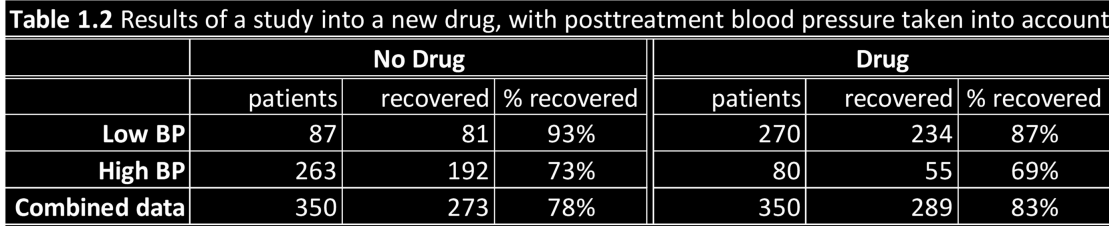
\includegraphics[width=0.6\textwidth]{immagini/simp_para_exe2.png}
    \caption{Simpson's Paradox - Second Example.}
    \label{fig:simp_para_exe2.png}
\end{figure}

\section{Ladder of Causation}
\subsubsection{Level of Association}
Prediction based on passive observations, for instace an marketing director asking if a customer
who bought a toothpase is likely to buy a toothbrush.
\subsubsection{Level of Intervention}
Actionable predictions based on interventions, for instance, a marketing director asking if a customer
is likely to buy a toothbrush if offered a discount.
\subsubsection{Level of Counterfactual}
Predictions based on hypothetical outcomes of events that happened in the past. 
For instance, a marketing director asking if a customer would have bought a toothbrush if he had not bought a toothpaste.

\chapter{Potential Outcomes Framework}
\section{Individual Treatment Effect}
\textbf{
SISTEMARE FORMULE, HO UNA MAREA DI FORMULE RIPETUTE
LE ASSUMPTION POSSONO DIVENTARE DELL DEF
}
Before going into the formal definition of the individual treatment effect,
we need to introduce some notation:
\begin{itemize}
    \item $X$ it's the random variable for \textbf{Treatment} (most of the time binary)
    \item $Y$ it's the random variable for \textbf{Outcome}, also called the \textbf{observed outcome} (most of the time binary)
    \item $Z$ it's a set of random variables for \textbf{Covariates}
    \item $Y(x)$ it's the \textbf{potential outcome} if the treatment $X=x$ is applied
    \item $X_i, Y_i, Z_i$ are the realizations of the random variables $X, Y, Z$ for the $i$-th individual in the population 
\end{itemize}
In general, the uppercase letters are used to denote random variables,
while the lowercase letters are used to denote their realizations.
\newline
For example, consider the case in which we have:
\begin{itemize}
    \item Happiness as the outcome variable $Y$
    \item Dog as the treatment variable $X$
    \item Y(1) the potential outcome of happiness if the individual gets a dog (X=1)
    \item Y(0) the potential outcome of happiness if the individual does not get a dog (X=0)
\end{itemize}
we could have the scenarios observed in \ref{fig:pot_out_scenarios}
\begin{figure}[H]
    \centering
    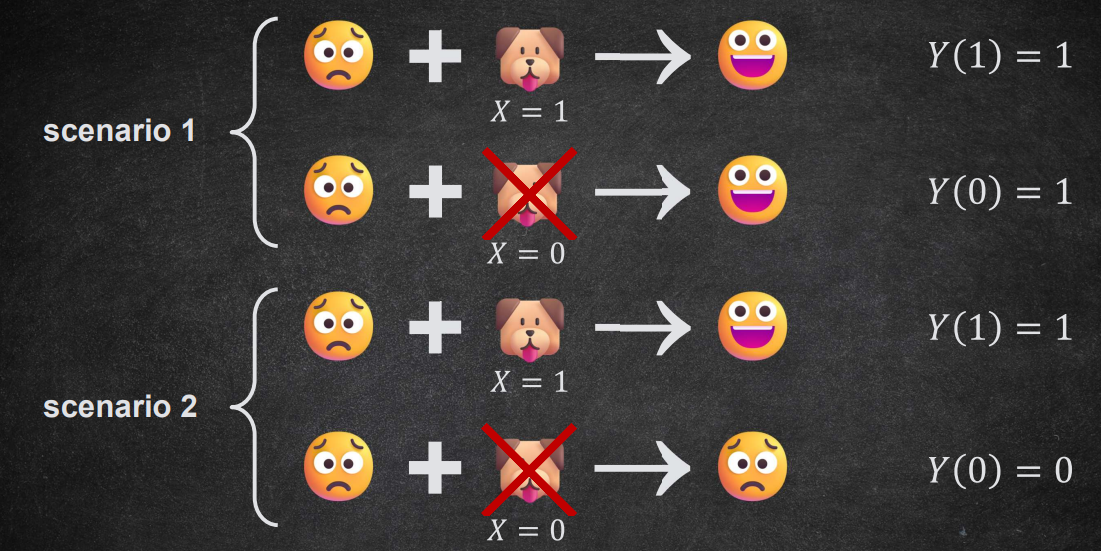
\includegraphics[width=0.7\textwidth]{immagini/pot_out_scenarios.png}
    \caption{Individual Treatment Effect}
    \label{fig:pot_out_scenarios}
\end{figure}
\noindent
It's important to point out that:
\begin{itemize}
    \item $Y(x)$ is distinct from $Y$ because not all potential outcomes are 
    observed, although all potential outcomes could be observed.
    \item The actually observed potential outcome depends on the given value x of treatment $X$.
\end{itemize} 
Of course, in reality the population is composed of many individuals or units,
every one of which is associated with one or more variables ($Z$).
\newline
\begin{definition}[Individual treatment effect (ITE)]
    for the $i^{th}$ individual is defined as the difference between the potential outcome for the treatment
    $X = 1$ and the potential outcome for the treatment $X = 0$:
    \begin{equation}
        \tau_i \triangleq Y_i(1) - Y_i(0)
    \end{equation} 
\end{definition}
\noindent
It is one of the main quantities of interest in causal inference. Y(x) is a random variable, 
while $Y_i(x)$ is treated as non-random because it is restricted to a specific individual
whose potential outcomes are deterministic.
This is a theoretical/conceptual definition because, as we said before, we can only observe one 
of the two potential outcomes for each individual. This leads us to the \textbf{Fundamental Problem of Causal Inference}. 
\section{The Fundamental Problem of Causal Inference}
If we consider the example of the dog and happiness, we can see that an individual can't get a dog,
observe Y(1), give the dog away and then observe Y(0). The second observation will be influenced by
all the action taken between the two observations.
\footnote{ML cares only about predicting Y, so ML does not have to deal with the fundamental problem of causal inference.}
There are others two definitions:
\begin{itemize}
    \item \textbf{Counterfactual}: potential outcomes that aren't (and can't be) observed
    \item \textbf{Factual}: potential outcomes that are observed
\end{itemize}
Note that there are no counterfactuals or factuals until the outcome is observed.
\newline
What helps us solve this problem is the average of treatment effect.
\begin{definition}[Average Treatment Effect (ATE)]
    obtained by taking an average over the ITEs
    \begin{equation}
        \tau \triangleq E[\tau_i] = E[Y_i(1) - Y_i(0)] = E[Y(1) - Y(0)]
        \label{eq:ate_init}
    \end{equation}
\end{definition}
\noindent
Let now us consider a population of 6 individuals, with the data shown in Table \ref{tab:potential_outcomes}. 
The fundamental problem of causal inference can be seen as a \textbf{Missing Data Problem} where the question
marks (?) mean that we do not observe the value for the corresponding cell.
\begin{table}[htbp]
    \centering
    \begin{tabular}{cccccc}
        \toprule
        $i$ & $X$ & $Y$ & $Y(1)$ & $Y(0)$ & $Y(1) - Y(0)$ \\
        \midrule
        1 & 0 & 0 & ? & 0 & ? \\
        2 & 1 & 1 & 1 & ? & ? \\
        3 & 1 & 0 & 0 & ? & ? \\
        4 & 0 & 0 & ? & 0 & ? \\
        5 & 0 & 1 & ? & 1 & ? \\
        6 & 1 & 1 & 1 & ? & ? \\
        \bottomrule
    \end{tabular}
    \caption{Potential Outcomes and Missing Data}
    \label{tab:potential_outcomes}
\end{table}
So the problem here is that we cannot compute the ATE (or ACE) directly because of missing 
counterfactual values.
Furthermore, we cannot simply rely on the \textbf{Associational Difference}:
$$\mathbb{E}[Y \vert{} X = 1] - \mathbb{E}[Y \vert{} X = 0]$$
because it compares two distinct subpopulations ($X=1$ vs $X=0$) rather than the same individuals 
under both conditions, indeed it isn't a causal quantity.
However we can rewrite the formula \ref{eq:ate_init} by using linear properties of expectation\footnote{
For any random variables $A$ and $B$ and constants $a, b \in \mathbb{R}$: $\mathbb{E}[aA + bB] = a\mathbb{E}[A] + b\mathbb{E}[B]$
\noindent
regardless of whether $A$ and $B$ are independent or dependent
}:
\begin{equation}
    \tau \triangleq \mathbb{E}[\tau_i] = \mathbb{E}[Y(1) - Y(0)] = \mathbb{E}[Y(1)] - \mathbb{E}[Y(0)]
\end{equation}
The \textit{associational difference} and the formulation of the ATE we just obtained are not equal
due to \textbf{confounding}. In Figure \ref{fig:confouning_graph} is depicted how the covariate $Z$ confounds
the effect of $X$ on $Y$, if we pay attention is also the graph of variables of Simpson's paradox example showed in Cap \ref{simp_para_cap}.
\begin{figure}[htbp]
    \centering
    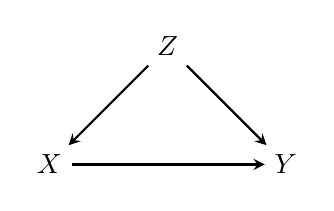
\begin{tikzpicture}[
        node/.style={circle, fill=green!60!black, text=white, minimum size=8mm, inner sep=0pt, font=\large\bfseries},
        arrow/.style={-stealth, thick, white}
    ]
        % Definizione dei nodi disposti a triangolo
        \node (Z) at (0, 1.5) {$Z$};
        \node (X) at (-1.5, 0) {$X$};
        \node (Y) at (1.5, 0) {$Y$};

        % Frecce direzionali
        \draw[->, thick, >=stealth] (Z) -- (X);
        \draw[->, thick, >=stealth] (Z) -- (Y);
        \draw[->, thick, >=stealth] (X) -- (Y);
    \end{tikzpicture}
    \caption{Causation between variables}
    \label{fig:confouning_graph}
\end{figure}
\newline
In conclusion  we can't \textbf{in general} compare the \textit{associational difference} with the \textit{ATE} due to confounding.
However there are some \textit{assumption} under which the equality holds true:
\begin{equation}
    \tau \triangleq \mathbb{E}[\tau_i] = \mathbb{E}[Y(1)] - \mathbb{E}[Y(0)] = \mathbb{E}[Y \vert{} X = 1] - \mathbb{E}[Y \vert{} X = 0]
    \label{eq:asso_equal_ate}
\end{equation}

\section{Assumptions for ATE}
As discussed, the Fundamental Problem of Causal Inference presents itself as a 
\textbf{missing data problem}, preventing us from directly computing the ATE. 
To bridge the gap between theoretical potential outcomes and observable data, 
we must rely on a set of core identifying assumptions centered around the concept of ignorability.
\newline
\begin{definition}[Ignorability / Exchangeability]
Ignorability states that the potential outcomes are independent of the treatment assignment:
\[
\left(Y(1), Y(0)\right) \perp\!\!\!\perp X
\]
It means that we can ignore how individuals ended up selecting treatment $X$. In terms of populations, the groups are \emph{exchangeable} in the sense that if their treatment assignments were swapped, the new treatment group would observe the same outcome distribution as the old treatment group, and vice versa.
\end{definition}
So we don't consider the causality between $X$ and $Z$ as shown in Fig \ref{fig:ignorability_graph}
\begin{figure}[htbp]
    \centering
    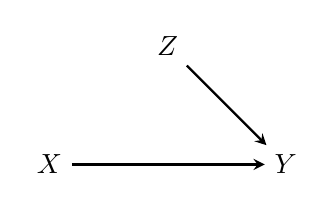
\begin{tikzpicture}[
        node/.style={circle, fill=green!60!black, text=white, minimum size=8mm, inner sep=0pt, font=\large\bfseries},
        arrow/.style={-stealth, thick, white}
    ]
        % Definizione dei nodi disposti a triangolo
        \node (Z) at (0, 1.5) {$Z$};
        \node (X) at (-1.5, 0) {$X$};
        \node (Y) at (1.5, 0) {$Y$};

        % Frecce direzionali
        \draw[->, thick, >=stealth] (Z) -- (Y);
        \draw[->, thick, >=stealth] (X) -- (Y);
    \end{tikzpicture}
    \caption{Causation between variables}
    \label{fig:ignorability_graph}
\end{figure}
\newline
This assumption alone allows us to use the formula \ref{eq:asso_equal_ate}\footnote{Strictly speaking,
the weaker assumption of \emph{Mean Ignorability} (or mean exchangeability, 
constraining only the first moment of the distribution: $\mathbb{E}[Y(1)\mid X=x] = \mathbb{E}[Y(1)]$)
would be sufficient for the ATE. However, it is standard practice to assume complete (full) 
ignorability as defined here.} and it also guarantees that the groups are comparable ($X=1$ and $X=0$ are
the same in all relevant aspects other than the treatment $X$).
\newline
Another aspect in which this assumption is crucial is that it allows us to \textbf{identify causal effects}, in other words, it satisfies the property of \textbf{Identifiability}:
\begin{definition}[Identifiability]
A causal quantity (e.g., $\mathbb{E}[Y(x)]$) is identifiable if it can be computed exclusively from purely statistical quantities derived from observational data (e.g., $\mathbb{E}[Y \mid X = x]$).
\end{definition}
However, making this assumption in observational studies is often \textbf{unrealistic} 
(or a strong identifying assumption). In practice, unobserved confounders frequently invalidate 
full ignorability, which is why conditioning on observed covariates $Z$ (conditional ignorability) 
becomes necessary.
\begin{definition}[Unconfoundedness / Conditional Exchangeability]
    conditional on a set of observed covariates, the treatment is independent of the potential outcomes:
    \begin{equation}
        \left(Y(1), Y(0)\right) \perp\!\!\!\perp X | Z
    \end{equation}
\end{definition}
This means that although the treatment and potential outcomes may be unconditionally associated
(due to confounding), within levels of Z, they are not associated. The 
\textit{non-causal association $X \leftarrow Z \rightarrow Y$}
is blocked at Z by conditioning on Z (X and Y are d-separated by Z).
\newline
With this new assumption the \ref{eq:asso_equal_ate} becomes:
\begin{equation}
    \tau \triangleq \mathbb{E}[\tau_i] = \mathbb{E}[Y(1)|Z] - \mathbb{E}[Y(0)|Z] = \mathbb{E}[Y \vert{} X = 1,Z] - \mathbb{E}[Y \vert{} X = 0,Z]
\end{equation}
\newline
There may be some unobserved confounders ($W$ as shown in Figure \ref{fig:confounder_w}) that 
are not part of the observed covariate set $Z = \{M\}$, meaning that 
\textbf{unconfoundedness is violated}. Fortunately, this is typically not an issue in ideal 
\textbf{randomized experiments}. However, it remains a critical challenge that we must always 
account for when working with \textbf{observational data}. Intuitively, the best practice is to observe and adjust for as many relevant covariates 
in $Z$ as possible to support the unconfoundedness assumption. However, as we will explore in 
subsequent lectures, conditioning on more covariates does not automatically yield less biased 
causal estimates. 
In fact, adjusting for the ``wrong covariates'' 
(e.g., conditioning on $N$ in $Z = \{M, N\}$ as illustrated in Figure \ref{fig:wrong_covariate_n}) can actually 
introduce or increase estimation bias. Specifically, adjusting for $M$ provides unbiased estimates, 
whereas adjusting for $N$ results in biased estimates.
\begin{figure}[htbp]
    \centering
    \begin{subfigure}[b]{0.45\textwidth}
        \centering
        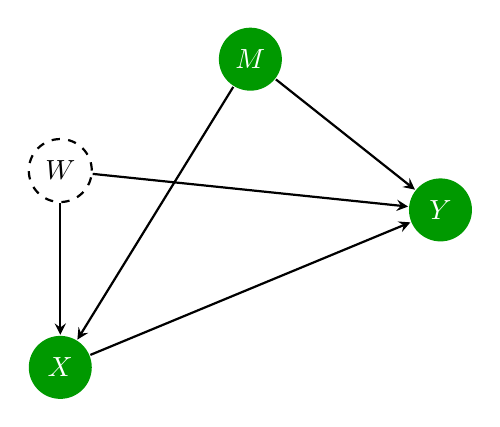
\begin{tikzpicture}[->, >=stealth, node distance=2cm, thick, main node/.style={circle, fill=green!60!black, text=white, minimum size=8mm}, unobserved node/.style={circle, draw=black, dashed, minimum size=8mm}]
            % Nodes
            \node[unobserved node] (W) {$W$};
            \node[main node] (M) [above right of=W, xshift=1cm] {$M$};
            \node[main node] (X) [below of=W, yshift=-0.5cm] {$X$};
            \node[main node] (Y) [below right of=M, xshift=1cm, yshift=-0.5cm] {$Y$};
            
            % Edges
            \draw (W) -- (X);
            \draw (W) -- (Y);
            \draw (M) -- (X);
            \draw (M) -- (Y);
            \draw (X) -- (Y);
        \end{tikzpicture}
        \caption{Unobserved Confounder $W$}
        \label{fig:confounder_w}
    \end{subfigure}
    \hfill
    \begin{subfigure}[b]{0.45\textwidth}
        \centering
        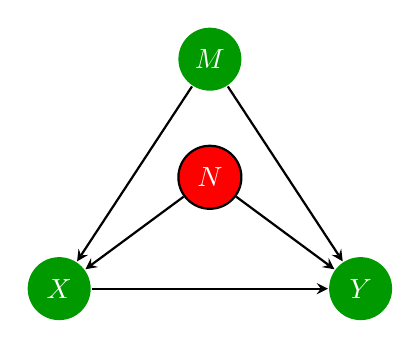
\begin{tikzpicture}[->, >=stealth, node distance=2cm, thick, main node/.style={circle, fill=green!60!black, text=white, minimum size=8mm}, bad node/.style={circle, fill=red, draw=black, text=white, minimum size=8mm}]
            % Nodes
            \node[main node] (M) {$M$};
            \node[bad node] (N) [below of=M, yshift=0.5cm] {$N$};
            \node[main node] (X) [below left of=N, xshift=-0.5cm] {$X$};
            \node[main node] (Y) [below right of=N, xshift=0.5cm] {$Y$};
            
            % Edges
            \draw (M) -- (X);
            \draw (M) -- (Y);
            \draw (N) -- (X);
            \draw (N) -- (Y);
            \draw (X) -- (Y);
        \end{tikzpicture}
        \caption{Wrong Covariate $N$}
        \label{fig:wrong_covariate_n}
    \end{subfigure}
    \caption{Comparison between an unobserved confounder $W$ and a problematic covariate adjustment $N$.}
    \label{fig:dag_comparisons}
\end{figure}
\noindent
Conditioning on many covariates is attractive for achieving unconfoundedness, but it can be 
detrimental for another reason that has to do with positivity.
\begin{definition}[Positivity / Overlap / Common Support]
    For all values $\bm{z}$ of covariates $\bm{Z}$ present in the population of interest (i.e., $\bm{z}$ such that $P(\bm{Z} = \bm{z}) > 0$):
    \begin{equation}
        0 < P(X = 1 \mid \bm{Z} = \bm{z}) < 1
    \end{equation}
    In other words, is the condition that all subgroups of the data with different value for covariates
    have some probability of receiving any value of treatment.
\end{definition}
\begin{remark}[Positivity Violation Leads to Division by Zero]
if we rewrite the right-hand side of 
\[
\mathbb{E}[Y(1) - Y(0)] = \mathbb{E}_{\mathbf{Z}}[\mathbb{E}[Y \mid X = 1, \mathbf{Z}] - \mathbb{E}[Y \mid X = 0, \mathbf{Z}]]
\]
in the case of discrete covariate variables $\mathbf{Z}$, to obtain:
\begin{align*}
    &= \sum_{\mathbf{z}} P(\mathbf{Z} = \mathbf{z}) \left( \sum_{y} y \, P(Y = y \mid X = 1, \mathbf{Z} = \mathbf{z}) - \sum_{y} y \, P(Y = y \mid X = 0, \mathbf{Z} = \mathbf{z}) \right) \\
    &= \sum_{\mathbf{z}} P(\mathbf{Z} = \mathbf{z}) \left( \sum_{y} y \frac{P(Y = y, X = 1, \mathbf{Z} = \mathbf{z})}{P(X = 1 \mid \mathbf{Z} = \mathbf{z}) P(\mathbf{Z} = \mathbf{z})} - \sum_{y} y \frac{P(Y = y, X = 0, \mathbf{Z} = \mathbf{z})}{P(X = 0 \mid \mathbf{Z} = \mathbf{z}) P(\mathbf{Z} = \mathbf{z})} \right)
\end{align*}
As we can observe from the denominators in the final expression, if the positivity assumption 
is violated for some value $\mathbf{z}$ (meaning $P(X = 1 \mid \mathbf{Z} = \mathbf{z}) = 0$ 
or $P(X = 0 \mid \mathbf{Z} = \mathbf{z}) = 0$), the expression results in a division by zero, 
making the causal effect undefined for that stratum. This makes positivity essential to define causal 
effect.
\end{remark}

\textbf{SLIDE 39}




\begin{definition}[Adjustment Formula]
    Given the assumptions of unconfoundedness, positivity, consistency,
    and no interference, we can identify the ATE:
    \begin{equation}
        \tau \triangleq E[\tau_i] = \mathbb{E_Z}[\mathbb{E}[Y \vert{} X = 1,Z] - \mathbb{E}[Y \vert{} X = 0,Z]]
    \end{equation}
\end{definition}


\chapter{Flow of Association and Causation Graphs}
\textbf{VALUTARE SE METTERE GRAFICI}


\section{Graph Concepts}
A \textbf{Graph} is a collection of \textbf{nodes} (vertices) and \textbf{edges}.
\begin{definition}[Adjacent nodes]
    Two nodes are adjacent if there is an edge between them    
\end{definition}
\begin{definition}[Complete graph]
    A graph is complete if there is an edge between every pair of nodes   
\end{definition}
\begin{definition}[Directed graph]
    A graph is directed\footnote{orientato} if the all his edges are directed   
\end{definition}
In a directed graph we can see some sets of nodes, based on the relationships showed by the edges:
\begin{itemize}
    \item \textbf{pa(X)} is the parent set of X
    \item \textbf{ch(Y)} is the child set of Y
    \item \textbf{de(Y)} is the descendants of Y, that is the set of nodes which can be reached by Y
    \item \textbf{an(Z)} is the set of ancestors of Z, the set of nodes from which Z can be reached.
\end{itemize}
It is also important to distinguish between a \textbf{Path}, that is any sequence of adjacent nodes, 
regardless of the direction of the edges that join them, and a \textbf{Directed Path}, that is a path
between two nodes traced along the arrows. So as a conseguence, in a directed path it can't be any node
on the path that has two edges on the path directed into it or out of it.
\newline
\section{From PGMs to CGMs}
The \textit{Probabilitstic Grapical models} are statistical models more often represented by 
\textbf{Bayesian Networks} in which we want to study the associations or the correlations between 
variables by modelling the \textbf{Data Distribution}:
\begin{definition}[Chain Rule]
    \begin{equation}
        \begin{aligned}
            P(X_1, X_2, \dots, X_n) &= P(X_1) P(X_2 \mid X_1) P(X_3 \mid X_1, X_2) \cdots P(X_n \mid X_1, \dots, X_{n-1}) \\
            &= P(X_1) \prod_{i=2}^{n} P(X_i \mid X_1, \dots, X_{i-1})
        \end{aligned}
    \end{equation}
\end{definition}

\end{document}
